\documentclass{beamer}\usepackage[]{graphicx}\usepackage[]{xcolor}
% maxwidth is the original width if it is less than linewidth
% otherwise use linewidth (to make sure the graphics do not exceed the margin)
\makeatletter
\def\maxwidth{ %
  \ifdim\Gin@nat@width>\linewidth
    \linewidth
  \else
    \Gin@nat@width
  \fi
}
\makeatother

\definecolor{fgcolor}{rgb}{0.345, 0.345, 0.345}
\newcommand{\hlnum}[1]{\textcolor[rgb]{0.686,0.059,0.569}{#1}}%
\newcommand{\hlstr}[1]{\textcolor[rgb]{0.192,0.494,0.8}{#1}}%
\newcommand{\hlcom}[1]{\textcolor[rgb]{0.678,0.584,0.686}{\textit{#1}}}%
\newcommand{\hlopt}[1]{\textcolor[rgb]{0,0,0}{#1}}%
\newcommand{\hlstd}[1]{\textcolor[rgb]{0.345,0.345,0.345}{#1}}%
\newcommand{\hlkwa}[1]{\textcolor[rgb]{0.161,0.373,0.58}{\textbf{#1}}}%
\newcommand{\hlkwb}[1]{\textcolor[rgb]{0.69,0.353,0.396}{#1}}%
\newcommand{\hlkwc}[1]{\textcolor[rgb]{0.333,0.667,0.333}{#1}}%
\newcommand{\hlkwd}[1]{\textcolor[rgb]{0.737,0.353,0.396}{\textbf{#1}}}%
\let\hlipl\hlkwb

\usepackage{framed}
\makeatletter
\newenvironment{kframe}{%
 \def\at@end@of@kframe{}%
 \ifinner\ifhmode%
  \def\at@end@of@kframe{\end{minipage}}%
  \begin{minipage}{\columnwidth}%
 \fi\fi%
 \def\FrameCommand##1{\hskip\@totalleftmargin \hskip-\fboxsep
 \colorbox{shadecolor}{##1}\hskip-\fboxsep
     % There is no \\@totalrightmargin, so:
     \hskip-\linewidth \hskip-\@totalleftmargin \hskip\columnwidth}%
 \MakeFramed {\advance\hsize-\width
   \@totalleftmargin\z@ \linewidth\hsize
   \@setminipage}}%
 {\par\unskip\endMakeFramed%
 \at@end@of@kframe}
\makeatother

\definecolor{shadecolor}{rgb}{.97, .97, .97}
\definecolor{messagecolor}{rgb}{0, 0, 0}
\definecolor{warningcolor}{rgb}{1, 0, 1}
\definecolor{errorcolor}{rgb}{1, 0, 0}
\newenvironment{knitrout}{}{} % an empty environment to be redefined in TeX

\usepackage{alltt}
\usepackage{graphicx}

\usepackage{graphicx}
\usepackage{verbatim}
\usepackage{etoolbox}
\usepackage{everysel}
% \usepackage{enumitem}

%% This package allows text highlighting
\usepackage{soul}

%% This sets the theme of the presentation which controls
%% the formatting of the slides
\usetheme{Boadilla}

%% Turn off the navigation symbols
\setbeamertemplate{navigation symbols}{} 

%% Change the default itemize [ball]s to [circle]s
\setbeamertemplate{itemize items}[circle]

%% Change the default enumerate [ball]s to plain text
\setbeamertemplate{enumerate items}[default]

%% Load the enumitem package and ensure it works nicely with beamer
% \setitemize{label=\usebeamerfont*{itemize item}
%   \usebeamercolor[fg]{itemize item}
%   \usebeamertemplate{itemize item}}
% \setenumerate{label=\usebeamerfont*{enumerate item}
%   \usebeamercolor[fg]{enumerate item}
%   \usebeamertemplate{enumerate item}}

%% Set the author block so STATS 201/8 appears on every
\author{STATS 201/8}

%% Clear the date block
\date{}


\setbeamercolor{title}{bg=blue!40}
\setbeamerfont{title}{size=\LARGE,series=\bfseries}

%%Sectioning commands
\setbeamercolor{section title}{bg=blue!20}
\setbeamerfont{section title}{size=\large}

\setbeamertemplate{section page}{%
    \begingroup
        \begin{beamercolorbox}[sep=10pt,center,rounded=true,shadow=true]{section title}
        \usebeamerfont{section title}Section~\thechapter.\thesection \newline \insertsection\par
        \end{beamercolorbox}
		\vfill
    \endgroup
}

\newcommand{\BeginSection}[1]{\section{#1} \frame{\sectionpage}}
%\AtBeginSection[]{%
%    \begin{frame}
%        \sectionpage
%    \end{frame}
%}


%% This makes all equations blue
\AtBeginEnvironment{equation*}{\color{blue}}
\AtBeginEnvironment{align*}{\color{blue}}
\everymath{\color{blue}}

%% This puts a 0 point space between paragraphs, means we don't need to use vspace, or list environments if 
%% we don't want to
\setlength{\parskip}{0pt}


%% Russell: removes spaces after R input/output?
\setlength{\topsep}{0.5mm}

%% David: In addition to Russel's command to remove spaces after R input/output, these commands remove the space between R input/output.
%% Stackoverflow link: https://stackoverflow.com/questions/35734525/reduce-space-between-code-chunks-and-code-output-in-rmarkdown-beamer-presentatio
%% \setlength{\OuterFrameSep}{-2pt}
\makeatletter
\preto{\@verbatim}{\topsep=-1pt \partopsep=-1pt }
\makeatother

%% Some useful colors
\definecolor{darkgreen}{rgb}{0.176,0.486,0.031}
\definecolor{redbrown}{HTML}{950605}
\definecolor{darkred}{HTML}{d80605}


%% nice little macro for changing the font of R code
\newcommand{\rcode}[1]{\protect{\color{darkgreen}\texttt{#1}}}

%% macro for bold blue italics
\newcommand{\blueBoldEmph}[1]{{\color{blue}\textbf{\emph{#1}}}}

% ~iid macro
\newcommand{\iid }{\stackrel{iid}{\sim}}

%% Macro for t-test amd P-value
\newcommand{\ttest}{\emph{t}-test}
\newcommand{\pval}{\emph{P}-value}

%% Statistics operators 
\DeclareMathOperator{\Bias}{Bias}
\DeclareMathOperator{\Cov}{Cov}
\DeclareMathOperator*{\Cor}{Cor}
\DeclareMathOperator{\E}{E}
\DeclareMathOperator{\MSE}{MSE}
\DeclareMathOperator{\Odds}{Odds}
\DeclareMathOperator{\OR}{OR}
\DeclareMathOperator{\PMSE}{PMSE}
\DeclareMathOperator{\sd}{sd}
\DeclareMathOperator{\se}{se}
\DeclareMathOperator*{\Var}{Var}
\DeclareMathOperator{\logit}{logit}

%% Should see if can make this a mathop
\newcommand{\comb}[2]{\mbox{$\big(_{#2}^{#1}\big)$}}






\IfFileExists{upquote.sty}{\usepackage{upquote}}{}
\begin{document}
\newcommand{\thechapter}{10}

\title{Chapter 10: Multiple linear regression models}
\institute{University of Auckland}


\begin{frame}
\titlepage
\end{frame}


\begin{frame}[t]
\frametitle{Learning Outcomes}
In this chapter you will learn about:
\begin{center}
\vspace{16pt}
\begin{minipage}{0.9\textwidth}
  \begin{itemize}
  \item Models with several explanatory variables
  \item Exploring pairwise relationships between all variables
  \item Multiple linear regression and the problem of multi-collinearity
  \item Fixing multi-collinearity
  \item Relevant \rcode{R}-code.
  \end{itemize}
\end{minipage}
\end{center}

\end{frame}


%%%%%%%%%%%%%%%%%%%%%%%%%%%%%%%%%%%%%%%%%%%%%%%%%%%%%%%%%%%%%%%%%%%%%%%%%%%%%%%%%%%%%%%%%%%
\BeginSection{Example: Modelling birth weights using several explanatory variables}
%%%%%%%%%%%%%%%%%%%%%%%%%%%%%%%%%%%%%%%%%%%%%%%%%%%%%%%%%%%%%%%%%%%%%%%%%%%%%%%%%%%%%%%%%%%


\begin{frame}
  \frametitle{Multiple explanatory variables }
  We have learned how to model the effects of numeric and/or factor explanatory variables using linear models.\\
  \bigskip
  More generally, we can (in principle) fit as many explanatory variables as we like. However, we shall see that this is not always a good idea.\\
  \bigskip
  Caution needs to be applied.\\
  \bigskip
  By way of example, let us examine which variables might explain the birth weight of babies.\\
\end{frame}



\begin{frame}[fragile]
\frametitle{Example: Birth weight of babies}
\begin{tabular}{ll }

   \rcode{bwt}            & birth weight in ounces (=28.35gm) \\
   \rcode{gestation}      & length of pregnancy in days  \\
   \rcode{not.first.born} & 0=first born, 1=not first-born\\
   \rcode{age}            & mother's age in years \\
   \rcode{height}         & mother's height in inches \\
   \rcode{weight}         & mother's pre-pregnancy weight in pounds \\
   \rcode{smoke}          & smoking status of mother  0=not, 1=smoker.

\end{tabular}
\medskip

The response variable is the baby's birth weight (\rcode{bwt}).
\bigskip

This dataset\footnote{It accompanies the excellent text Stat Labs: Mathematical Statistics through Applications Springer-Verlag (2001) by Deborah Nolan and Terry Speed.} was obtained from
\href{http://www.stat.berkeley.edu/users/statlabs/labs.html}{http://www.stat.berkeley.edu/users/statlabs/labs.html}.
\medskip

The dataset has 1174 observations.
\end{frame}


%%%%%%%%%%%%%%%%%%%%%%%%%%%%%%%%%%%%%%%%%%%%%%%%%%%%%%%%%%%%%%%%%%%%%%%%%%%%%%%%%%%%%%%%%%%
\BeginSection{Exploring relationships between the variables}
%%%%%%%%%%%%%%%%%%%%%%%%%%%%%%%%%%%%%%%%%%%%%%%%%%%%%%%%%%%%%%%%%%%%%%%%%%%%%%%%%%%%%%%%%%%


\begin{frame}[fragile]
\frametitle{Birth weight of babies}
% note code gets rid of white space by pretending to submit but doing it `on the sly' later
Let us first inspect the relationships between the numerical explanatory variables and the response variable. 
The numeric explanatories are \rcode{gestation}, \rcode{age}, \rcode{height}   and \rcode{weight}. 

\bigskip
The five variables are in columns 1,2,4,5  and 6 in the data frame \rcode{Babies.df}.

\bigskip
\begin{knitrout}\scriptsize
\definecolor{shadecolor}{rgb}{0.969, 0.969, 0.969}\color{fgcolor}\begin{kframe}
\begin{alltt}
\hlstd{> }\hlcom{## Invoke the s20x library}
\hlstd{> }\hlkwd{library}\hlstd{(s20x)}
\hlstd{> }\hlcom{## Importing data into R}
\hlstd{> }\hlstd{Babies.df} \hlkwb{=} \hlkwd{read.table}\hlstd{(}\hlstr{"Data/babies_data.txt"}\hlstd{,} \hlkwc{header}\hlstd{=T)}
\hlstd{> }\hlcom{## Create the pairs plot of the five numeric variables}
\hlstd{> }\hlkwd{pairs20x}\hlstd{(Babies.df[,}\hlkwd{c}\hlstd{(}\hlnum{1}\hlstd{,}\hlnum{2}\hlstd{,}\hlnum{4}\hlstd{,}\hlnum{5}\hlstd{,}\hlnum{6}\hlstd{)])}
\end{alltt}
\end{kframe}
\end{knitrout}
\end{frame}


\begin{frame}[fragile]
\frametitle{Birth weight of babies\ldots}
\begin{knitrout}\scriptsize
\definecolor{shadecolor}{rgb}{0.969, 0.969, 0.969}\color{fgcolor}\begin{kframe}


{\ttfamily\noindent\color{warningcolor}{Warning in par(usr): argument 1 does not name a graphical parameter}}

{\ttfamily\noindent\color{warningcolor}{Warning in par(usr): argument 1 does not name a graphical parameter}}

{\ttfamily\noindent\color{warningcolor}{Warning in par(usr): argument 1 does not name a graphical parameter}}

{\ttfamily\noindent\color{warningcolor}{Warning in par(usr): argument 1 does not name a graphical parameter}}

{\ttfamily\noindent\color{warningcolor}{Warning in par(usr): argument 1 does not name a graphical parameter}}

{\ttfamily\noindent\color{warningcolor}{Warning in par(usr): argument 1 does not name a graphical parameter}}

{\ttfamily\noindent\color{warningcolor}{Warning in par(usr): argument 1 does not name a graphical parameter}}

{\ttfamily\noindent\color{warningcolor}{Warning in par(usr): argument 1 does not name a graphical parameter}}

{\ttfamily\noindent\color{warningcolor}{Warning in par(usr): argument 1 does not name a graphical parameter}}

{\ttfamily\noindent\color{warningcolor}{Warning in par(usr): argument 1 does not name a graphical parameter}}

{\ttfamily\noindent\color{warningcolor}{Warning in par(usr): argument 1 does not name a graphical parameter}}

{\ttfamily\noindent\color{warningcolor}{Warning in par(usr): argument 1 does not name a graphical parameter}}

{\ttfamily\noindent\color{warningcolor}{Warning in par(usr): argument 1 does not name a graphical parameter}}

{\ttfamily\noindent\color{warningcolor}{Warning in par(usr): argument 1 does not name a graphical parameter}}

{\ttfamily\noindent\color{warningcolor}{Warning in par(usr): argument 1 does not name a graphical parameter}}\end{kframe}
\end{knitrout}
\begin{figure}
  \centering
  \includegraphics[scale = 0.45]{figure/RC-H10-002}
\end{figure}

\end{frame}


\begin{frame}[fragile]
\frametitle{Birth weight of babies\ldots}
\rcode{pairs20x} gives a histogram of each variable in the diagonal cells. 
Above the diagonal, in the $(i,j)$ cell ($i<j$) it gives scatter plots of variable $i$ (y-axis) against variable $j$ (x-axis).
To illustrate, variable 1 is \rcode{bwt} and variable 4 is the mother's height (\rcode{height}). The scatter plot in cell (1,4) is

\begin{knitrout}\scriptsize
\definecolor{shadecolor}{rgb}{0.969, 0.969, 0.969}\color{fgcolor}\begin{kframe}
\begin{alltt}
\hlstd{> }\hlkwd{plot}\hlstd{(bwt} \hlopt{~} \hlstd{height,}\hlkwc{data} \hlstd{= Babies.df)}
\hlstd{> }\hlkwd{lines}\hlstd{(}\hlkwd{lowess}\hlstd{(Babies.df}\hlopt{$}\hlstd{height,Babies.df}\hlopt{$}\hlstd{bwt))}
\end{alltt}
\end{kframe}
\end{knitrout}



\begin{figure}
  \centering
  \includegraphics{figure/RC-H10-004}
\end{figure}

\end{frame}


\begin{frame}[fragile]
\frametitle{Birth weight of babies\ldots}
The correlation coefficient between \rcode{height} and \rcode{bwt} is in cell (4,1).
It is $0.20$, indicating that a straight-line relationship is, at best, weak.\\
\bigskip
This correlation coefficient can only measure the strength of a straight line relationship between $x$ (\rcode{height}) and a $y$ (\rcode{bwt}). It can be useful but can, on occasion, be misleading.
In other words, look at the scatter plot and use it only if the relationship looks like a straight line.\\
\bigskip
\textbf{Note:} In a simple linear regression of $y$ on $x$, the resulting $R^2$ value is the square of the sample correlation coefficient. To illustrate:

\medskip
\begin{knitrout}\scriptsize
\definecolor{shadecolor}{rgb}{0.969, 0.969, 0.969}\color{fgcolor}\begin{kframe}
\begin{alltt}
\hlstd{> }\hlkwd{summary}\hlstd{(}\hlkwd{lm}\hlstd{(bwt} \hlopt{~} \hlstd{height,}\hlkwc{data} \hlstd{= Babies.df))}\hlopt{$}\hlstd{r.squared}
\end{alltt}
\begin{verbatim}
[1] 0.04149539
\end{verbatim}
\begin{alltt}
\hlstd{> }\hlkwd{cor}\hlstd{(Babies.df}\hlopt{$}\hlstd{bwt,Babies.df}\hlopt{$}\hlstd{height)}\hlopt{^}\hlnum{2}
\end{alltt}
\begin{verbatim}
[1] 0.04149539
\end{verbatim}
\end{kframe}
\end{knitrout}
\end{frame}


\begin{frame}[fragile]
\frametitle{Birth weight of babies\ldots}
Looking at the pairs plot again, we also see a somewhat weak relationship between \rcode{bwt} and mother's \rcode{weight}.
\medskip

\begin{knitrout}\scriptsize
\definecolor{shadecolor}{rgb}{0.969, 0.969, 0.969}\color{fgcolor}\begin{kframe}
\begin{alltt}
\hlstd{> }\hlkwd{plot}\hlstd{(bwt} \hlopt{~} \hlstd{weight,}\hlkwc{data} \hlstd{= Babies.df)}
\hlstd{> }\hlkwd{lines}\hlstd{(}\hlkwd{lowess}\hlstd{(Babies.df}\hlopt{$}\hlstd{weight,Babies.df}\hlopt{$}\hlstd{bwt))}
\end{alltt}
\end{kframe}
\end{knitrout}



\begin{figure}
  \centering
  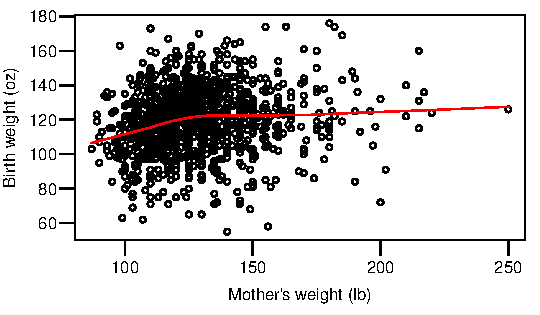
\includegraphics{figure/RC-H10-007}
\end{figure}

\end{frame}


\begin{frame}[fragile]
\frametitle{Birth weight of babies\ldots}

There is a stronger relationship between the \rcode{gestation} time for the babies and its \rcode{bwt} which is not surprising, as the longer the child is in the mother's womb the longer the child has had time to have nutrition and grow.
But, this relationship distinctly flattens out beyond a certain gestational age -- some people call this a ``hockey stick'' curve.

\begin{knitrout}\scriptsize
\definecolor{shadecolor}{rgb}{0.969, 0.969, 0.969}\color{fgcolor}\begin{kframe}
\begin{alltt}
\hlstd{> }\hlkwd{plot}\hlstd{(bwt} \hlopt{~} \hlstd{gestation,}\hlkwc{data} \hlstd{= Babies.df)}
\hlstd{> }\hlkwd{lines}\hlstd{(}\hlkwd{lowess}\hlstd{(Babies.df}\hlopt{$}\hlstd{gestation,Babies.df}\hlopt{$}\hlstd{bwt))}
\end{alltt}
\end{kframe}
\end{knitrout}
%identify(Babies.df$gestation,Babies.df$bwt)



\begin{figure}
  \centering
  \includegraphics{figure/RC-H10-009}
\end{figure}

\end{frame}


\begin{frame}[fragile]
\frametitle{Birth weight of babies\ldots}

There does not seem to be any relationship between a mother's age  and her child's \rcode{bwt}.

\begin{knitrout}\scriptsize
\definecolor{shadecolor}{rgb}{0.969, 0.969, 0.969}\color{fgcolor}\begin{kframe}
\begin{alltt}
\hlstd{> }\hlkwd{plot}\hlstd{(bwt} \hlopt{~} \hlstd{age,}\hlkwc{data} \hlstd{= Babies.df)}
\hlstd{> }\hlkwd{lines}\hlstd{(}\hlkwd{lowess}\hlstd{(Babies.df}\hlopt{$}\hlstd{age,Babies.df}\hlopt{$}\hlstd{bwt))}
\end{alltt}
\end{kframe}
\end{knitrout}



\begin{figure}
  \centering
  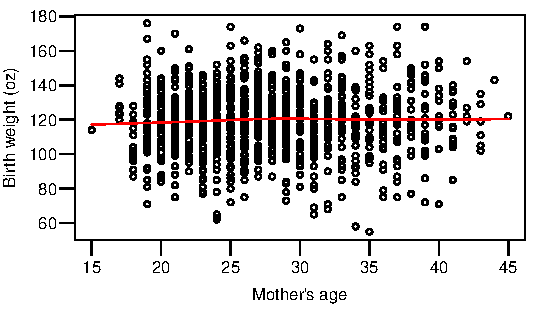
\includegraphics{figure/RC-H10-011}
\end{figure}

\end{frame}

\begin{frame}
\frametitle{Birth weight of babies\ldots}

\textbf{Note:} There seem to be some outlying data points in these plots.
There does not appear to be much of a relationship between the $x$ variables, except between \rcode{height} and \rcode{weight}.
\medskip

\begin{figure}
  \centering
  \includegraphics[scale = 0.3]{figure/RC-H10-002}
\end{figure}

\end{frame}


\begin{frame}[fragile]
\frametitle{Birth weight of babies\ldots}
Let us look at the categorical (factor) explanatory variables against the baby's birth weight \rcode{bwt}.

The categorical variables are \rcode{not.first.born} and \rcode{smoke},
in columns 3 and 7 of the data frame \rcode{Babies.df}.

\begin{knitrout}\scriptsize
\definecolor{shadecolor}{rgb}{0.969, 0.969, 0.969}\color{fgcolor}\begin{kframe}
\begin{alltt}
\hlstd{> }\hlkwd{pairs20x}\hlstd{(Babies.df[,}\hlkwd{c}\hlstd{(}\hlnum{1}\hlstd{,}\hlnum{3}\hlstd{,}\hlnum{7}\hlstd{)])}
\end{alltt}


{\ttfamily\noindent\color{warningcolor}{Warning in par(usr): argument 1 does not name a graphical parameter}}

{\ttfamily\noindent\color{warningcolor}{Warning in par(usr): argument 1 does not name a graphical parameter}}

{\ttfamily\noindent\color{warningcolor}{Warning in par(usr): argument 1 does not name a graphical parameter}}

{\ttfamily\noindent\color{warningcolor}{Warning in par(usr): argument 1 does not name a graphical parameter}}

{\ttfamily\noindent\color{warningcolor}{Warning in par(usr): argument 1 does not name a graphical parameter}}

{\ttfamily\noindent\color{warningcolor}{Warning in par(usr): argument 1 does not name a graphical parameter}}\end{kframe}
\end{knitrout}

\begin{knitrout}\scriptsize
\definecolor{shadecolor}{rgb}{0.969, 0.969, 0.969}\color{fgcolor}\begin{kframe}


{\ttfamily\noindent\color{warningcolor}{Warning in par(usr): argument 1 does not name a graphical parameter}}

{\ttfamily\noindent\color{warningcolor}{Warning in par(usr): argument 1 does not name a graphical parameter}}

{\ttfamily\noindent\color{warningcolor}{Warning in par(usr): argument 1 does not name a graphical parameter}}

{\ttfamily\noindent\color{warningcolor}{Warning in par(usr): argument 1 does not name a graphical parameter}}

{\ttfamily\noindent\color{warningcolor}{Warning in par(usr): argument 1 does not name a graphical parameter}}

{\ttfamily\noindent\color{warningcolor}{Warning in par(usr): argument 1 does not name a graphical parameter}}\end{kframe}
\end{knitrout}

\begin{figure}
  \centering
  \includegraphics[scale = 0.3]{figure/RC-H10-013}
\end{figure}

\end{frame}


\begin{frame}[fragile]
\frametitle{Birth weight of babies\ldots}
We see a slight decrease in babies \rcode{bwt} if the mother smokes. This increases the chance of a mother having a low birth weight baby if she smokes -- perhaps another reason to avoid tobacco!\\
\bigskip
The variable \rcode{not.first.born} does not appear to have too much of an effect. This is perhaps not a surprise given that this variable may not be as important as it once was as family size has deceased markedly in the developed world (this is US data) and prenatal care has improved.\\
\bigskip

We will know begin our linear modelling of these data...
\end{frame}


\begin{frame}[fragile]
\frametitle{Birth weight of babies\ldots}
\framesubtitle{Relationship between birth weight and gestational age}
Let us start with an understanding of \rcode{gestation} to explain \rcode{bwt} since it is
the strongest relationship. The atypical data points have been marked with question marks.
We will add other explanatory variables later.
%with(Babies.df,identify(gestation,bwt))
\begin{knitrout}\scriptsize
\definecolor{shadecolor}{rgb}{0.969, 0.969, 0.969}\color{fgcolor}\begin{kframe}
\begin{alltt}
\hlstd{> }\hlkwd{plot}\hlstd{(bwt} \hlopt{~} \hlstd{gestation,}\hlkwc{data} \hlstd{= Babies.df)}
\hlstd{> }\hlkwd{lines}\hlstd{(}\hlkwd{lowess}\hlstd{(Babies.df}\hlopt{$}\hlstd{gestation, Babies.df}\hlopt{$}\hlstd{bwt),} \hlkwc{col} \hlstd{=} \hlstr{"red"}\hlstd{)}
\hlstd{> }\hlkwd{text}\hlstd{(}\hlkwd{c}\hlstd{(}\hlnum{152}\hlstd{,} \hlnum{185}\hlstd{),}\hlkwd{c}\hlstd{(}\hlnum{120}\hlstd{,} \hlnum{115}\hlstd{),} \hlstr{"?"}\hlstd{,} \hlkwc{col} \hlstd{=} \hlstr{"red"}\hlstd{)}
\hlstd{> }\hlkwd{abline}\hlstd{(}\hlkwc{v} \hlstd{=} \hlnum{294}\hlstd{,}\hlkwc{lty} \hlstd{=} \hlnum{3}\hlstd{)}
\end{alltt}
\end{kframe}
\end{knitrout}



\begin{figure}
  \centering
  \includegraphics{figure/RC-H10-015}
\end{figure}
\end{frame}


\begin{frame}[fragile]
\frametitle{Birth weight of babies\ldots}
\framesubtitle{Relationship between birth weight and gestational age\ldots}
Let us identify the two points denoted by the `?' symbol.\\
\bigskip
We can easily identify them in the plot as they have $\rcode{gestation}<200$.\\
\bigskip
They look extremely implausible as they have typical birth-weight but have a gestational age that is extremely low for these data.\\
\bigskip
\begin{knitrout}\scriptsize
\definecolor{shadecolor}{rgb}{0.969, 0.969, 0.969}\color{fgcolor}\begin{kframe}
\begin{alltt}
\hlstd{> }\hlstd{id}\hlkwb{=}\hlstd{(Babies.df}\hlopt{$}\hlstd{gestation}\hlopt{<}\hlnum{200}\hlstd{)}
\hlstd{> }\hlstd{Babies.df[id,]}
\end{alltt}
\begin{verbatim}
    bwt gestation not.first.born age height weight smokes
239 116       148              0  28     66    135      0
820 110       181              0  27     64    133      0
\end{verbatim}
\end{kframe}
\end{knitrout}
\bigskip
These points (observations 239 and 820) may be be unduly influential.
\end{frame}


\begin{frame}[fragile]
\frametitle{Birth weight of babies\ldots}
\framesubtitle{Relationship between birth weight and gestational age\ldots}
The above plot has a vertical line at 294 days. The relevance of 294 days is explained in the article \href{https://goo.gl/k8XbSd}{\underline{``How Your Baby Grows During Pregnancy''}}.\\
\medskip

Most babies are born before 42 weeks = $42 \times 7 =294$ days. It seems that beyond this point babies cease to grow and hence the `flattening out' and/or decrease. In other words, it looks like the effect of gestational age depends on whether the baby is overdue or not. That is, the effect of gestational age appears to change with overdue status.
\bigskip

We want to fit a model that fits a straight line for $\rcode{gestation} \le 294$ and then changes the slope of that line when $\rcode{gestation}>294$.

\begin{columns}
\begin{column}{0.7\textwidth}
{\color{black} We'll need to put our statistical thinking caps on, and devise a way to fit such a model.}
\end{column}
\begin{column}{0.3\textwidth}

\includegraphics[width=1.0in]{ThinkingCap3.jpg}
\end{column}
\end{columns}

\end{frame}



\begin{frame}[fragile]
\frametitle{Birth weight of babies\ldots}
\framesubtitle{Relationship between birth weight and gestational age\ldots}
For $\rcode{gestation} \le 294$ days we'll use the familiar simple linear regression model
\[
\E[\rcode{bwt}]=\beta_0 + \rcode{gestation} \times \beta_1
\]
\vspace{-1ex}

We'd like to extend this model by adding an extra term so that the slope changes when $\rcode{gestation}>294$. That is,

\[
\E[\rcode{bwt}]=\beta_0 + \rcode{gestation} \times \beta_1 + v \times \beta_2
\]
where $v$ is some suitable explanatory variable. What should $v$ be? 
\medskip

\begin{itemize}
\item For $\rcode{gestation} \le 294$ the extended model is just the simple linear regression model, so that means $v=0$ when $\rcode{gestation} \le 294$.
\item For $\rcode{gestation} > 294$ we need another slope effect for gestational age. In fact, we need $v = \rcode{gestation} - 294$.\footnote{We substract the 294 so that the simple linear regression model and extended model have the same value when $\rcode{gestation} = 294$, because then $v=0$.}
\end{itemize}

\end{frame}


\begin{frame}[fragile]
\frametitle{Birth weight of babies\ldots}
\framesubtitle{Relationship between birth weight and gestational age\ldots}
Let's create the new explanatory $v = \rcode{gestation} - 294$ that is described above. We'll give it the name \rcode{ODdays} because it is the number of days that the baby is overdue.

\begin{knitrout}\scriptsize
\definecolor{shadecolor}{rgb}{0.969, 0.969, 0.969}\color{fgcolor}\begin{kframe}
\begin{alltt}
\hlstd{> }\hlkwd{head}\hlstd{(Babies.df,}\hlnum{12}\hlstd{)} \hlcom{#Print first 12 lines of dataframe}
\end{alltt}
\begin{verbatim}
   bwt gestation not.first.born age height weight smokes ODdays
1  120       284              0  27     62    100      0      0
2  113       282              0  33     64    135      0      0
3  128       279              0  28     64    115      1      0
4  108       282              0  23     67    125      1      0
5  136       286              0  25     62     93      0      0
6  138       244              0  33     62    178      0      0
7  132       245              0  23     65    140      0      0
8  120       289              0  25     62    125      0      0
9  143       299              0  30     66    136      1      5
10 140       351              0  27     68    120      0     57
11 144       282              0  32     64    124      1      0
12 141       279              0  23     63    128      1      0
\end{verbatim}
\end{kframe}
\end{knitrout}
\end{frame}



%%%%%%%%%%%%%%%%%%%%%%%%%%%%%%%%%%%%%%%%%%%%%%%%%%%%%%%%%%%%%%%%%%%%%%%%%%%%%%%%%%%%%%%%%%%
\BeginSection{Fitting the initial model}
%%%%%%%%%%%%%%%%%%%%%%%%%%%%%%%%%%%%%%%%%%%%%%%%%%%%%%%%%%%%%%%%%%%%%%%%%%%%%%%%%%%%%%%%%%%


\begin{frame}[fragile]
\frametitle{Birth weight of babies\ldots}
Our initial fitted model is the hockey stick model for the effect of gestational age.
\begin{knitrout}\scriptsize
\definecolor{shadecolor}{rgb}{0.969, 0.969, 0.969}\color{fgcolor}\begin{kframe}
\begin{alltt}
\hlstd{> }\hlstd{bwt.fit}\hlkwb{=}\hlkwd{lm}\hlstd{(bwt}\hlopt{~} \hlstd{gestation}\hlopt{+}\hlstd{ODdays,} \hlkwc{data} \hlstd{= Babies.df)}
\hlstd{> }\hlkwd{plot}\hlstd{(bwt.fit,} \hlkwc{which} \hlstd{=} \hlnum{1}\hlstd{,} \hlkwc{add.smooth} \hlstd{=} \hlnum{FALSE}\hlstd{)}
\end{alltt}
\end{kframe}
\end{knitrout}


\begin{figure}
  \centering
  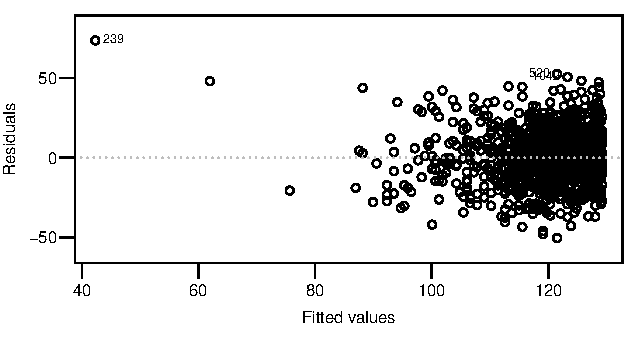
\includegraphics{figure/RC-H10-020}
\end{figure}

Observation 239 is a problem.
\end{frame}


\begin{frame}[fragile]
\frametitle{Birth weight of babies\ldots}
\begin{knitrout}\scriptsize
\definecolor{shadecolor}{rgb}{0.969, 0.969, 0.969}\color{fgcolor}\begin{kframe}
\begin{alltt}
\hlstd{> }\hlkwd{normcheck}\hlstd{(bwt.fit)}
\end{alltt}
\end{kframe}
\end{knitrout}



\begin{figure}
  \centering
  \includegraphics[scale = 0.5]{figure/RC-H10-022}
\end{figure}

Other than observation 239, things look pretty good.
\end{frame}


\begin{frame}[fragile]
\frametitle{Birth weight of babies\ldots}
\begin{knitrout}\scriptsize
\definecolor{shadecolor}{rgb}{0.969, 0.969, 0.969}\color{fgcolor}\begin{kframe}
\begin{alltt}
\hlstd{> }\hlkwd{cooks20x}\hlstd{(bwt.fit)}
\end{alltt}
\end{kframe}
\end{knitrout}



\begin{figure}
  \centering
  \includegraphics[scale = 0.5]{figure/RC-H10-024}
\end{figure}

Point 239 is unduly influential. 
This baby has a gestational age of just 148 days, and yet has a weight typical of a full term baby. It is clearly a data-entry mistake and we will remove this data point.
\end{frame}


\begin{frame}[fragile]
\frametitle{Birth weight of babies\ldots}
Let us refit with observation 239 removed.
\begin{knitrout}\scriptsize
\definecolor{shadecolor}{rgb}{0.969, 0.969, 0.969}\color{fgcolor}\begin{kframe}
\begin{alltt}
\hlstd{> }\hlstd{bwt.fit2}\hlkwb{=}\hlkwd{lm}\hlstd{(bwt}\hlopt{~} \hlstd{gestation}\hlopt{+}\hlstd{ODdays,}\hlkwc{data} \hlstd{= Babies.df[}\hlopt{-}\hlnum{239}\hlstd{,])}
\hlstd{> }\hlkwd{cooks20x}\hlstd{(bwt.fit2)}
\end{alltt}
\end{kframe}
\end{knitrout}



\begin{figure}
  \centering
  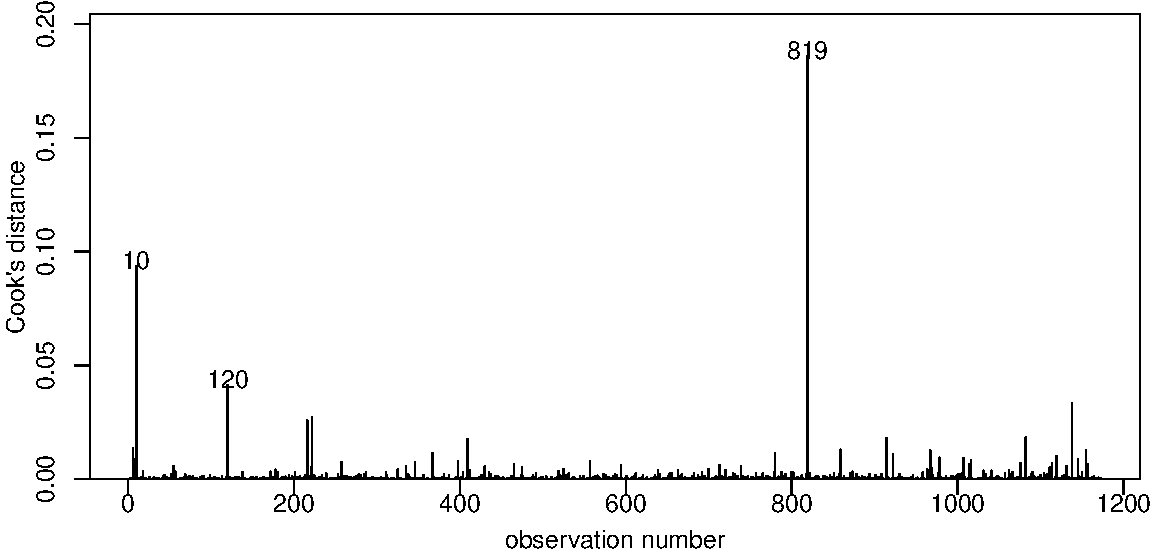
\includegraphics[scale = 0.5]{figure/RC-H10-026}
\end{figure}

Although observation 820~\footnote{Note that it is now identified as point 819 in this plot, but it was point 820 before we dropped point 239.} is not unduly influential,
but we shall make a judgement call, and remove it.
\end{frame}


\begin{frame}[fragile]
\frametitle{Birth weight of babies\ldots}
We refit the model using the reduced data.

\begin{knitrout}\scriptsize
\definecolor{shadecolor}{rgb}{0.969, 0.969, 0.969}\color{fgcolor}\begin{kframe}
\begin{alltt}
\hlstd{> }\hlcom{#This time we demonstrate using the subset argument to remove points}
\hlstd{> }\hlstd{bwt.fit3}\hlkwb{=}\hlkwd{lm}\hlstd{(bwt}\hlopt{~} \hlstd{gestation}\hlopt{+}\hlstd{ODdays,}\hlkwc{data} \hlstd{= Babies.df,} \hlkwc{subset} \hlstd{=} \hlopt{-}\hlkwd{c}\hlstd{(}\hlnum{239}\hlstd{,} \hlnum{820}\hlstd{))}
\hlstd{> }\hlkwd{cooks20x}\hlstd{(bwt.fit3)}
\end{alltt}
\end{kframe}
\end{knitrout}



\begin{figure}
  \centering
  \includegraphics[scale = 0.5]{figure/RC-H10-028}
\end{figure}

Now we have no unduly influential data points.
\end{frame}



\begin{frame}[fragile]
\frametitle{Birth weight of babies\ldots}
Let us recheck the residuals now that we have removed these two points.
\begin{knitrout}\scriptsize
\definecolor{shadecolor}{rgb}{0.969, 0.969, 0.969}\color{fgcolor}\begin{kframe}
\begin{alltt}
\hlstd{> }\hlkwd{plot}\hlstd{(bwt.fit3,}\hlkwc{which}\hlstd{=}\hlnum{1}\hlstd{)}
\end{alltt}
\end{kframe}
\end{knitrout}



\begin{figure}
  \centering
  \includegraphics{figure/RC-H10-030}
\end{figure}

EOV seems fine now, and the residuals seem to be centred around zero.
\end{frame}


\begin{frame}[fragile]
\frametitle{Birth weight of babies\ldots}
Let's take a look at our fitted hockey stick model.

\begin{knitrout}\scriptsize
\definecolor{shadecolor}{rgb}{0.969, 0.969, 0.969}\color{fgcolor}\begin{kframe}
\begin{alltt}
\hlstd{> }\hlstd{gestation.seq}\hlkwb{=}\hlnum{201}\hlopt{:}\hlnum{360} \hlcom{#Explanatory values at which to get predictions}
\hlstd{> }\hlstd{ODdays.seq}\hlkwb{=}\hlkwd{ifelse}\hlstd{(gestation.seq}\hlopt{<=}\hlnum{294}\hlstd{,}\hlnum{0}\hlstd{,gestation.seq}\hlopt{-}\hlnum{294}\hlstd{)}
\hlstd{> }\hlstd{fit.seq}\hlkwb{=}\hlkwd{predict}\hlstd{(bwt.fit3,}\hlkwc{new}\hlstd{=}\hlkwd{data.frame}\hlstd{(}\hlkwc{gestation}\hlstd{=gestation.seq,}
\hlstd{+ }                                        \hlkwc{ODdays}\hlstd{=ODdays.seq))}
\hlstd{> }\hlkwd{plot}\hlstd{(bwt}\hlopt{~}\hlstd{gestation,}\hlkwc{data}\hlstd{=Babies.df[}\hlopt{-}\hlkwd{c}\hlstd{(}\hlnum{239}\hlstd{,} \hlnum{820}\hlstd{),])}
\hlstd{> }\hlkwd{lines}\hlstd{(gestation.seq,fit.seq,}\hlkwc{col}\hlstd{=}\hlstr{"red"}\hlstd{);} \hlkwd{abline}\hlstd{(}\hlkwc{v}\hlstd{=}\hlnum{294}\hlstd{,}\hlkwc{lty}\hlstd{=}\hlnum{2}\hlstd{,}\hlkwc{col}\hlstd{=}\hlstr{"blue"}\hlstd{)}
\end{alltt}
\end{kframe}
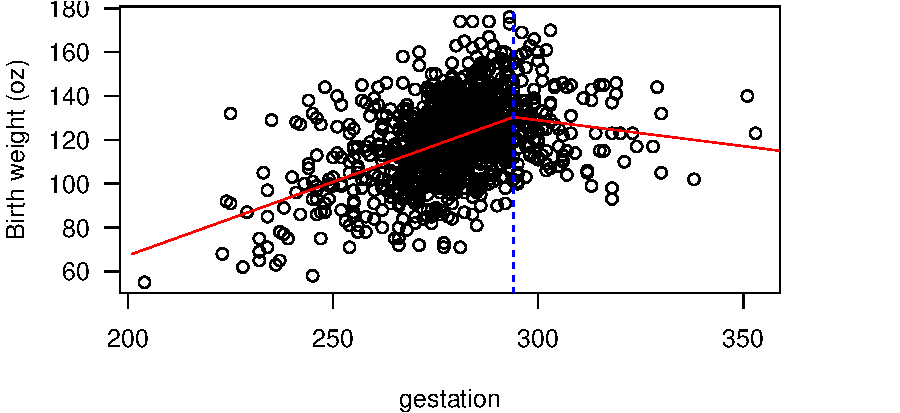
\includegraphics[width=\maxwidth]{figure/RC-H10-030_5-1} 
\end{knitrout}
\end{frame}



\begin{frame}[fragile]

Now we can trust this output let us interpret it.
\begin{knitrout}\scriptsize
\definecolor{shadecolor}{rgb}{0.969, 0.969, 0.969}\color{fgcolor}\begin{kframe}
\begin{alltt}
\hlstd{> }\hlkwd{summary}\hlstd{(bwt.fit3)}
\end{alltt}
\end{kframe}
\end{knitrout}

\begin{knitrout}\scriptsize
\definecolor{shadecolor}{rgb}{0.969, 0.969, 0.969}\color{fgcolor}\begin{kframe}
\begin{verbatim}
Coefficients:
             Estimate Std. Error t value Pr(>|t|)    
(Intercept) -66.95336   10.42810   -6.42 1.97e-10 ***
gestation     0.67124    0.03757   17.87  < 2e-16 ***
ODdays       -0.90783    0.11745   -7.73 2.31e-14 ***
---
Residual standard error: 16.23 on 1169 degrees of freedom
Multiple R-squared:  0.2188,	Adjusted R-squared:  0.2174 
F-statistic: 163.7 on 2 and 1169 DF,  p-value: < 2.2e-16
\end{verbatim}
\end{kframe}
\end{knitrout}

The fitted model is:
\[
 \E[\rcode{bwt}]=-66.95 + 0.67\times\rcode{gestation} -0.91\times\rcode{ODdays}  
\]
\end{frame}



\begin{frame}[fragile]
\frametitle{Birth weight of babies\ldots}
So, for $\rcode{gestation} \le 294$ days (i.e., \rcode{ODdays = 0})
\[
\E[\rcode{bwt}]=-66.95+0.67\times\rcode{gestation}
\]
That is, on average, babies initially grow at 0.67 oz per day until about 130 oz\footnote{
$130 \approx -66.95 + 0.67\times 294$} at week 42 (i.e., day 294).\\
\bigskip
For $\rcode{gestation} > 294$ days (i.e., \rcode{ODdays = gestation-294})
\begin{align*}
\E[\rcode{bwt}]&=-66.95+0.67\times\rcode{gestation}  -0.91\times(\rcode{gestation-294})\\
           &= 199.95 - 0.24\times\rcode{gestation}
\end{align*}

So, on average, it is estimated that overdue babies lose about 0.24 oz per day after week 42.\footnote{{\bf Question:} How could we test whether this is significantly different from zero?}
\end{frame}



\begin{frame}[fragile]
\frametitle{Birth weight of babies\ldots}
\textbf{Note} that this model only explains about 22\% of the variation in babies' birth weight, so it would be worth seeing if adding the other explanatory variables will help explain more.

\bigskip
In the \rcode{pairs20x} plot above we saw that \rcode{height} and \rcode{weight} had
correlations of 0.20 and 0.16 with \rcode{bwt}.

\bigskip
So let us see what we find when we introduce the \rcode{height} variable into the model. We will proceed with selecting variables one at a time (with reflection)  --  this is one of many multiple regression strategies!

\end{frame}


%%%%%%%%%%%%%%%%%%%%%%%%%%%%%%%%%%%%%%%%%%%%%%%%%%%%%%%%%%%%%%%%%%%%%%%%%%%%%%%%%%%%%%%%%%%
\BeginSection{Multiple linear regression model: \\ Adding more terms to the model and the peril of multi-collinearity}
%%%%%%%%%%%%%%%%%%%%%%%%%%%%%%%%%%%%%%%%%%%%%%%%%%%%%%%%%%%%%%%%%%%%%%%%%%%%%%%%%%%%%%%%%%%



\begin{frame}[fragile]
\frametitle{Birth weight of babies\ldots}
Let us add the \rcode{height} variable and see how it works out.
\begin{knitrout}\scriptsize
\definecolor{shadecolor}{rgb}{0.969, 0.969, 0.969}\color{fgcolor}\begin{kframe}
\begin{alltt}
\hlstd{> }\hlstd{bwt.fit4} \hlkwb{=} \hlkwd{lm}\hlstd{(bwt} \hlopt{~} \hlstd{gestation} \hlopt{+} \hlstd{ODdays} \hlopt{+} \hlstd{height,} \hlkwc{data} \hlstd{= Babies.df,}
\hlstd{+ }    \hlkwc{subset} \hlstd{=} \hlopt{-}\hlkwd{c}\hlstd{(}\hlnum{239}\hlstd{,}\hlnum{820}\hlstd{))}
\hlstd{> }\hlkwd{plot}\hlstd{(bwt.fit4,}\hlkwc{which}\hlstd{=}\hlnum{1}\hlstd{)}
\end{alltt}
\end{kframe}
\end{knitrout}



\begin{figure}
  \centering
  \includegraphics{figure/RC-H10-034}
\end{figure}

All seems okay. Let us make sure that this makes sense in terms of output.
\end{frame}



\begin{frame}[fragile]

\frametitle{Birth weight of babies\ldots}
\begin{knitrout}\scriptsize
\definecolor{shadecolor}{rgb}{0.969, 0.969, 0.969}\color{fgcolor}\begin{kframe}
\begin{alltt}
\hlstd{> }\hlkwd{summary}\hlstd{(bwt.fit4)}
\end{alltt}
\end{kframe}
\end{knitrout}

\begin{knitrout}\scriptsize
\definecolor{shadecolor}{rgb}{0.969, 0.969, 0.969}\color{fgcolor}\begin{kframe}
\begin{verbatim}
Coefficients:
              Estimate Std. Error t value Pr(>|t|)    
(Intercept) -139.20571   15.05961  -9.244  < 2e-16 ***
gestation      0.65219    0.03703  17.613  < 2e-16 ***
ODdays        -0.89039    0.11543  -7.714 2.61e-14 ***
height         1.21083    0.18495   6.547 8.79e-11 ***
---
Residual standard error: 15.94 on 1168 degrees of freedom
Multiple R-squared:  0.2464,	Adjusted R-squared:  0.2445 
F-statistic: 127.3 on 3 and 1168 DF,  p-value: < 2.2e-16
\end{verbatim}
\end{kframe}
\end{knitrout}
\bigskip
This seems to make sense, whereby mother's height is positively related to a baby's birth weight (on average).\\
\bigskip
\textbf{Note:} We will drop the checking of fitted vs residuals plots as it has been okay to date and it is starting to get a little tedious. We will recheck this once we get to the final model.
\end{frame}


\begin{frame}[fragile]
\frametitle{Birth weight of babies\ldots}
Let us add \rcode{weight} to the model. We're going to save some typing and use the \rcode{update} function to update our model.\footnote{In the above use of \rcode{update} the $~\tilde{} ~ .$ term is used to denote the model containing the explanatory variables in \rcode{bwt.fit4}.}
\medskip
\begin{knitrout}\scriptsize
\definecolor{shadecolor}{rgb}{0.969, 0.969, 0.969}\color{fgcolor}\begin{kframe}
\begin{alltt}
\hlstd{> }\hlstd{bwt.fit5} \hlkwb{=} \hlkwd{update}\hlstd{(bwt.fit4,}\hlopt{~}\hlstd{.} \hlopt{+} \hlstd{weight)}
\hlstd{> }\hlkwd{summary}\hlstd{(bwt.fit5)}
\end{alltt}
\end{kframe}
\end{knitrout}

\begin{knitrout}\scriptsize
\definecolor{shadecolor}{rgb}{0.969, 0.969, 0.969}\color{fgcolor}\begin{kframe}
\begin{verbatim}
Coefficients:
              Estimate Std. Error t value Pr(>|t|)    
(Intercept) -131.68169   15.14974  -8.692  < 2e-16 ***
gestation      0.65624    0.03688  17.795  < 2e-16 ***
ODdays        -0.90868    0.11502  -7.900 6.41e-15 ***
height         0.90486    0.20453   4.424 1.06e-05 ***
weight         0.08535    0.02485   3.434 0.000615 ***
---
Residual standard error: 15.87 on 1167 degrees of freedom
Multiple R-squared:  0.254,	Adjusted R-squared:  0.2514 
F-statistic: 99.32 on 4 and 1167 DF,  p-value: < 2.2e-16
\end{verbatim}
\end{kframe}
\end{knitrout}

This makes sense. Heavier mothers can be expected to have heavier babies.
\end{frame}


\begin{frame}[fragile]
\frametitle{Birth weight of babies\ldots}
The mother being very underweight or excessively overweight can have negative effects
on their babies health, but neither \rcode{height} or \rcode{weight} directly
measures this.\\
\bigskip
We will construct a new variable, body mass index \rcode{bmi}.\\
\bigskip
\[
BMI = \frac{\rcode{mass in kg}}{\rcode{height in metres}^2} =\frac{\rcode{mass in lb}}{\rcode{height in inches}^2}\times 703
\]

\bigskip
The World Health Organisation classifies BMIs in the range 18.5--25 as healthy,
25--30 as overweight, and 30+ as obese.
\end{frame}


\begin{frame}[fragile]
\frametitle{Birth weight of babies\ldots}
Let us add \rcode{bmi} to the current model.
\begin{knitrout}\scriptsize
\definecolor{shadecolor}{rgb}{0.969, 0.969, 0.969}\color{fgcolor}\begin{kframe}
\begin{alltt}
\hlstd{> }\hlcom{# Create the variable BMI and add it to the model}
\hlstd{> }\hlstd{Babies.df}\hlopt{$}\hlstd{bmi} \hlkwb{=} \hlstd{(Babies.df}\hlopt{$}\hlstd{weight} \hlopt{/} \hlstd{(Babies.df}\hlopt{$}\hlstd{height}\hlopt{^}\hlnum{2}\hlstd{) )} \hlopt{*} \hlnum{703}
\hlstd{> }\hlstd{bwt.fit6} \hlkwb{=} \hlkwd{update}\hlstd{(bwt.fit5,}\hlopt{~}\hlstd{.} \hlopt{+} \hlstd{bmi)}
\hlstd{> }\hlkwd{summary}\hlstd{(bwt.fit6)}
\end{alltt}
\end{kframe}
\end{knitrout}

\begin{knitrout}\scriptsize
\definecolor{shadecolor}{rgb}{0.969, 0.969, 0.969}\color{fgcolor}\begin{kframe}
\begin{verbatim}
Coefficients:
              Estimate Std. Error t value Pr(>|t|)    
(Intercept) -216.33575   79.63707  -2.717  0.00669 ** 
gestation      0.65629    0.03688  17.798  < 2e-16 ***
ODdays        -0.90980    0.11502  -7.910 5.94e-15 ***
height         2.22845    1.23940   1.798  0.07243 .  
weight        -0.24252    0.30382  -0.798  0.42490    
bmi            1.90870    1.76280   1.083  0.27914    
---
Residual standard error: 15.87 on 1166 degrees of freedom
Multiple R-squared:  0.2547,	Adjusted R-squared:  0.2515 
F-statistic:  79.7 on 5 and 1166 DF,  p-value: < 2.2e-16
\end{verbatim}
\end{kframe}
\end{knitrout}

Hang on. Everything has gone weird!!!
None of \rcode{weight}, \rcode{height} or \rcode{bmi} is statistically significant
(at the 5\% level). So what is going on?
\end{frame}



\begin{frame}[fragile]
\frametitle{Birth weight of babies\ldots}
Let's look at these three variables to see what is happening.
\begin{knitrout}\scriptsize
\definecolor{shadecolor}{rgb}{0.969, 0.969, 0.969}\color{fgcolor}\begin{kframe}
\begin{alltt}
\hlstd{> }\hlkwd{pairs20x}\hlstd{(Babies.df[}\hlopt{-}\hlkwd{c}\hlstd{(}\hlnum{239}\hlstd{,}\hlnum{820}\hlstd{),} \hlkwd{c}\hlstd{(}\hlnum{9}\hlstd{,}\hlnum{6}\hlstd{,}\hlnum{5}\hlstd{)])}
\end{alltt}


{\ttfamily\noindent\color{warningcolor}{Warning in par(usr): argument 1 does not name a graphical parameter}}

{\ttfamily\noindent\color{warningcolor}{Warning in par(usr): argument 1 does not name a graphical parameter}}

{\ttfamily\noindent\color{warningcolor}{Warning in par(usr): argument 1 does not name a graphical parameter}}

{\ttfamily\noindent\color{warningcolor}{Warning in par(usr): argument 1 does not name a graphical parameter}}

{\ttfamily\noindent\color{warningcolor}{Warning in par(usr): argument 1 does not name a graphical parameter}}

{\ttfamily\noindent\color{warningcolor}{Warning in par(usr): argument 1 does not name a graphical parameter}}\end{kframe}
\end{knitrout}

\begin{knitrout}\scriptsize
\definecolor{shadecolor}{rgb}{0.969, 0.969, 0.969}\color{fgcolor}\begin{kframe}


{\ttfamily\noindent\color{warningcolor}{Warning in par(usr): argument 1 does not name a graphical parameter}}

{\ttfamily\noindent\color{warningcolor}{Warning in par(usr): argument 1 does not name a graphical parameter}}

{\ttfamily\noindent\color{warningcolor}{Warning in par(usr): argument 1 does not name a graphical parameter}}

{\ttfamily\noindent\color{warningcolor}{Warning in par(usr): argument 1 does not name a graphical parameter}}

{\ttfamily\noindent\color{warningcolor}{Warning in par(usr): argument 1 does not name a graphical parameter}}

{\ttfamily\noindent\color{warningcolor}{Warning in par(usr): argument 1 does not name a graphical parameter}}\end{kframe}
\end{knitrout}

\begin{figure}
  \centering
  \includegraphics[scale = 0.35]{figure/RC-H10-042}
\end{figure}

Not surprisingly, we see that \rcode{bmi} and \rcode{weight} seem to explain each other.
\end{frame}


\begin{frame}[fragile]
\frametitle{Birth weight of babies\ldots}
The problem is that we have a redundancy in our explanatory variables.
Here, \rcode{bmi} is explained by \rcode{weight} and vice-versa.
Note that adding \rcode{bmi} to the model barely changed $R^2$ and so is telling us that it did not increase our ability to explain variability in birth weight.\\
\medskip
In essence the statistically significance (i.e., \pval{}) of an explanatory
variable is measuring its contribution toward explaining variability in the response variable (in our case \rcode{bwt})
\emph{having adjusted for any other explanatory variables in the model}.\\
\medskip
So \rcode{bmi} explains little variability in \rcode{bwt} since \rcode{weight} has already
explained most of that variability, and vice-versa.\\
\medskip
This problem is given the name \textbf{multi-collinearity}\footnote{The double `l' is not a mistake.}.\\
\medskip
In linear algebra, we say we have linear dependence (as opposed to linear independence) in these variables.
\end{frame}

\begin{frame}[fragile]
\frametitle{Birth weight of babies\ldots}
Back to the drawing board. Let us refit this model with \rcode{bmi} and \rcode{height}, but without \rcode{weight}.\\
\medskip
\begin{knitrout}\scriptsize
\definecolor{shadecolor}{rgb}{0.969, 0.969, 0.969}\color{fgcolor}\begin{kframe}
\begin{alltt}
\hlstd{> }\hlstd{bwt.fit7} \hlkwb{=} \hlkwd{update}\hlstd{(bwt.fit6,}\hlopt{~}\hlstd{.} \hlopt{-} \hlstd{weight)}
\hlstd{> }\hlkwd{summary}\hlstd{(bwt.fit7)}
\end{alltt}
\end{kframe}
\end{knitrout}

\begin{knitrout}\scriptsize
\definecolor{shadecolor}{rgb}{0.969, 0.969, 0.969}\color{fgcolor}\begin{kframe}
\begin{verbatim}
Coefficients:
              Estimate Std. Error t value Pr(>|t|)    
(Intercept) -153.99353   15.56725  -9.892  < 2e-16 ***
gestation      0.65633    0.03687  17.801  < 2e-16 ***
ODdays        -0.90933    0.11500  -7.907 6.06e-15 ***
height         1.25013    0.18440   6.779 1.91e-11 ***
bmi            0.50629    0.14415   3.512 0.000461 ***
---
Residual standard error: 15.87 on 1167 degrees of freedom
Multiple R-squared:  0.2543,	Adjusted R-squared:  0.2518 
F-statistic:  99.5 on 4 and 1167 DF,  p-value: < 2.2e-16
\end{verbatim}
\end{kframe}
\end{knitrout}

Let us next investigate whether the categorical variable (\rcode{smokes}) helps to
explain further variability in \rcode{bwt}.
\end{frame}



\begin{frame}[fragile]
\frametitle{Birth weight of babies\ldots}
Let us add \rcode{smokes} to this analysis.
\begin{knitrout}\scriptsize
\definecolor{shadecolor}{rgb}{0.969, 0.969, 0.969}\color{fgcolor}\begin{kframe}
\begin{alltt}
\hlstd{> }\hlstd{bwt.fit8}\hlkwb{=}\hlkwd{update}\hlstd{(bwt.fit7,}\hlopt{~}\hlstd{.} \hlopt{+} \hlstd{smokes)}
\hlstd{> }\hlkwd{summary}\hlstd{(bwt.fit8)}
\end{alltt}
\end{kframe}
\end{knitrout}

\begin{knitrout}\scriptsize
\definecolor{shadecolor}{rgb}{0.969, 0.969, 0.969}\color{fgcolor}\begin{kframe}
\begin{verbatim}
Coefficients:
              Estimate Std. Error t value Pr(>|t|)    
(Intercept) -144.07719   15.15079  -9.510  < 2e-16 ***
gestation      0.63198    0.03589  17.608  < 2e-16 ***
ODdays        -0.88104    0.11164  -7.892 6.84e-15 ***
height         1.28081    0.17898   7.156 1.46e-12 ***
bmi            0.41516    0.14029   2.959  0.00315 ** 
smokes        -7.93655    0.92711  -8.561  < 2e-16 ***
---
Residual standard error: 15.4 on 1166 degrees of freedom
Multiple R-squared:  0.2984,	Adjusted R-squared:  0.2954 
F-statistic: 99.18 on 5 and 1166 DF,  p-value: < 2.2e-16
\end{verbatim}
\end{kframe}
\end{knitrout}

As we might have suspected, a mother smoking is associated with decreased birth weight.
\end{frame}


\begin{frame}[fragile]
\frametitle{Birth weight of babies\ldots}
Let us see if \rcode{not.first.born} is useful:

\begin{knitrout}\scriptsize
\definecolor{shadecolor}{rgb}{0.969, 0.969, 0.969}\color{fgcolor}\begin{kframe}
\begin{alltt}
\hlstd{> }\hlstd{bwt.fit9}\hlkwb{=}\hlkwd{update}\hlstd{(bwt.fit8,}\hlopt{~}\hlstd{.} \hlopt{+} \hlstd{not.first.born)}
\hlstd{> }\hlkwd{summary}\hlstd{(bwt.fit9)}
\end{alltt}
\end{kframe}
\end{knitrout}

\begin{knitrout}\scriptsize
\definecolor{shadecolor}{rgb}{0.969, 0.969, 0.969}\color{fgcolor}\begin{kframe}
\begin{verbatim}
Coefficients:
                 Estimate Std. Error t value Pr(>|t|)    
(Intercept)    -145.56797   15.08855  -9.648  < 2e-16 ***
gestation         0.64129    0.03583  17.897  < 2e-16 ***
ODdays           -0.89215    0.11119  -8.024 2.48e-15 ***
height            1.29912    0.17825   7.288 5.78e-13 ***
bmi               0.35469    0.14078   2.520 0.011882 *  
smokes           -7.98201    0.92301  -8.648  < 2e-16 ***
not.first.born   -3.51137    1.02978  -3.410 0.000672 ***
---
Residual standard error: 15.33 on 1165 degrees of freedom
Multiple R-squared:  0.3053,	Adjusted R-squared:  0.3018 
F-statistic: 85.34 on 6 and 1165 DF,  p-value: < 2.2e-16
\end{verbatim}
\end{kframe}
\end{knitrout}
Hmmm, does the negative effect of \rcode{not.first.born} seem reasonable???
\end{frame}



\begin{frame}[fragile]
\frametitle{Birth weight of babies\ldots}
Let us check the assumptions on this final model:

Independence should be okay, as this is (hopefully) a random sample of data from
a carefully designed study.

\begin{knitrout}\scriptsize
\definecolor{shadecolor}{rgb}{0.969, 0.969, 0.969}\color{fgcolor}\begin{kframe}
\begin{alltt}
\hlstd{> }\hlkwd{plot}\hlstd{(bwt.fit9,}\hlkwc{which}\hlstd{=}\hlnum{1}\hlstd{)}
\end{alltt}
\end{kframe}
\end{knitrout}



\begin{figure}
  \centering
  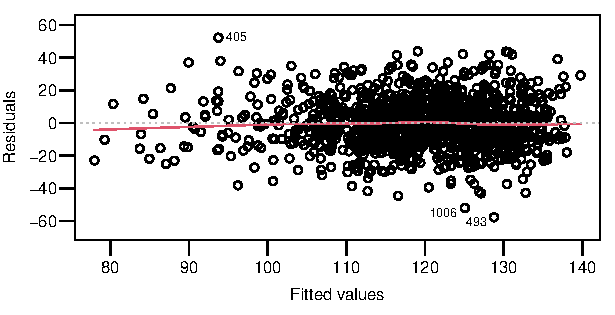
\includegraphics{figure/RC-H10-050}
\end{figure}

No trend, and EOV assumption is fine.
\end{frame}


\begin{frame}[fragile]
\frametitle{Birth weight of babies\ldots}
\begin{knitrout}\scriptsize
\definecolor{shadecolor}{rgb}{0.969, 0.969, 0.969}\color{fgcolor}\begin{kframe}
\begin{alltt}
\hlstd{> }\hlkwd{normcheck}\hlstd{(bwt.fit9)}
\end{alltt}
\end{kframe}
\end{knitrout}



\begin{figure}
  \centering
  \includegraphics[scale=0.5]{figure/RC-H10-052}
\end{figure}

Normality assumption looks fine.
\end{frame}


\begin{frame}[fragile]
\frametitle{Birth weight of babies\ldots}
\begin{knitrout}\scriptsize
\definecolor{shadecolor}{rgb}{0.969, 0.969, 0.969}\color{fgcolor}\begin{kframe}
\begin{alltt}
\hlstd{> }\hlkwd{cooks20x}\hlstd{(bwt.fit9)}
\end{alltt}
\end{kframe}
\end{knitrout}



\begin{figure}
  \centering
  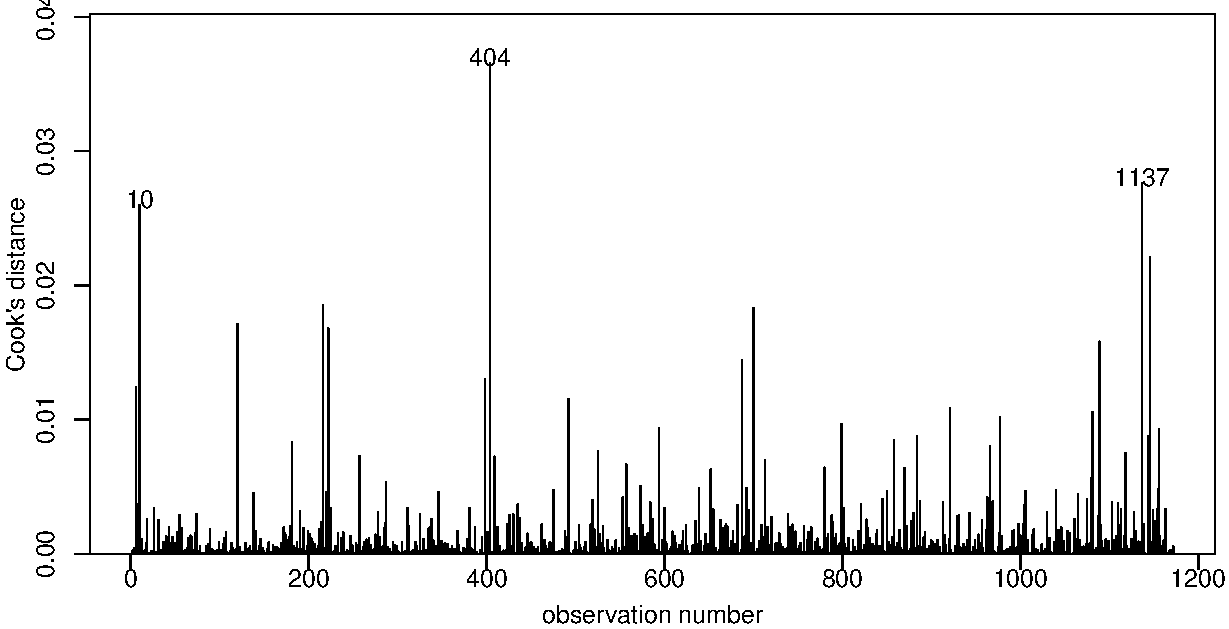
\includegraphics[scale=0.5]{figure/RC-H10-054}
\end{figure}

No unduly influential points.

\end{frame}



\begin{frame}[fragile,t]
\frametitle{Birth weight of babies\ldots}
Let us get the CIs on this trusted output. \\ 
\begin{knitrout}\scriptsize
\definecolor{shadecolor}{rgb}{0.969, 0.969, 0.969}\color{fgcolor}\begin{kframe}
\begin{alltt}
\hlstd{> }\hlkwd{confint}\hlstd{(bwt.fit9)}
\end{alltt}
\begin{verbatim}
                       2.5 %       97.5 %
(Intercept)    -175.17174865 -115.9641969
gestation         0.57098950    0.7115993
ODdays           -1.11029525   -0.6740001
height            0.94938608    1.6488470
bmi               0.07849275    0.6308947
smokes           -9.79295880   -6.1710576
not.first.born   -5.53179563   -1.4909493
\end{verbatim}
\end{kframe}
\end{knitrout}

\bigskip
See Case Study 10.1 for a  detailed  executive summary.\
\end{frame}



\begin{frame}[fragile]
\frametitle{Birth weight of babies\ldots}
\framesubtitle{Closing remarks}

Recall that we can fit as many explanatory variables as we like. So, did fitting all of these explanatory variables help us describe the variability of the birth weight of babies?

\medskip

{\renewcommand{\arraystretch}{1.15}

  \begin{tabular}{l|ll}
     & What we did & Multiple $R^2$ \\ \hline
    \rcode{bwt.fit3} & Added \rcode{gestation+ODdays} & 21.9\% \\
    \rcode{bwt.fit4} & Added \rcode{height} & 24.6\% \\
    \rcode{bwt.fit5} & Added \rcode{weight} & 25.4\% \\
    \rcode{bwt.fit6} & Added \rcode{bmi} & 25.5\% \\ 
    \rcode{bwt.fit7} & Dropped \rcode{weight} & 25.4\% \\
    \rcode{bwt.fit8} & Added \rcode{smokes} & 29.8\% \\
    \rcode{bwt.fit9} & Added \rcode{not.first.born} & 30.5\%
  \end{tabular}

}
\medskip

Our final model, \rcode{bwt.fit9}, includes explanatory variables we deemed suitable and it has a Multiple $R^2$ of 30.5\%. 

\end{frame}


%%%%%%%%%%%%%%%%%%%%%%%%%%%%%%%%%%%%%%%%%%%%%%%%%%%%%%%%%%%%%%%%%%%%%%%%%%%%%%%%%%%%%%%%%%%
\BeginSection{Closing remarks and relevant \rcode{R}-code}
%%%%%%%%%%%%%%%%%%%%%%%%%%%%%%%%%%%%%%%%%%%%%%%%%%%%%%%%%%%%%%%%%%%%%%%%%%%%%%%%%%%%%%%%%%%

\begin{frame}[fragile]
\frametitle{Closing remarks}

In situations where there are many explanatory variables,
some of which may be strongly correlated,
selecting the best subset for the final model can be challenging.
\bigskip

Model selection is a crucial component of statistical modelling and machine learning, especially in the context of ``big data'' where there may be millions of observations and thousands of potential explanatory variables.
\bigskip

STATS 330 (Advanced Statistical Modelling) covers this topic in more detail,
using techniques such as stepwise variable selection, AIC (Akaike's information criterion), and assessment of prediction error using cross validation.
\vfill
\end{frame}



\begin{frame}[fragile]
\frametitle{Most of the \rcode{R}-code you need for this chapter}

Note that this code comes with the usual code/checks discussed in chapters 1 and 2.
\medskip

Useful tools for inspecting many relationships are:

\begin{knitrout}\scriptsize
\definecolor{shadecolor}{rgb}{0.969, 0.969, 0.969}\color{fgcolor}\begin{kframe}
\begin{alltt}
\hlstd{> }\hlcom{## Create the pairs plot of the five numeric variables}
\hlstd{> }\hlkwd{pairs20x}\hlstd{(Babies.df[,}\hlkwd{c}\hlstd{(}\hlnum{1}\hlstd{,}\hlnum{2}\hlstd{,}\hlnum{4}\hlstd{,}\hlnum{5}\hlstd{,}\hlnum{6}\hlstd{)])}
\end{alltt}
\end{kframe}
\end{knitrout}

and for the factor variables:

\begin{knitrout}\scriptsize
\definecolor{shadecolor}{rgb}{0.969, 0.969, 0.969}\color{fgcolor}\begin{kframe}
\begin{alltt}
\hlstd{> }\hlkwd{pairs20x}\hlstd{(Babies.df[,}\hlkwd{c}\hlstd{(}\hlnum{1}\hlstd{,}\hlnum{3}\hlstd{,}\hlnum{7}\hlstd{)])}
\end{alltt}
\end{kframe}
\end{knitrout}
\medskip

Then it is a process of repeatedly updating the model and using Occam's razor to determine a preferred model. E.g.,
\begin{knitrout}\scriptsize
\definecolor{shadecolor}{rgb}{0.969, 0.969, 0.969}\color{fgcolor}\begin{kframe}
\begin{alltt}
\hlstd{> }\hlstd{model2}\hlkwb{=}\hlkwd{update}\hlstd{(model1,} \hlopt{~}\hlstd{.} \hlopt{+} \hlstd{xvariable2)}
\end{alltt}
\end{kframe}
\end{knitrout}

This requires constant vigilance to avoid multi-collinearity
\bigskip

Also note that some times several different models may be selected that all make sense and are acceptable.  
\end{frame}

\end{document}
